\section*{g) Analysis of runtime}

The analysis of the runtime is done in three steps, the check, the filtering step and the brute-force step. 

The check is parts 1. and 2. in the algorithm. The edges are sorted in $O(m\log m)$ time and then a minimum spanning tree is found using Kruskal's algorithm. This is repeated where the edges are sorted by their mirror's weight. In total, this takes $O(m\log m)$ time. 

The filtering step is polynomial in runtime. Here, for each edge in the graph, the edge is removed and a connectivity check is made, after which the edge is put back. The connectivity check is done in $O(\log^2(n))$ time. In total, this step takes $O(m\log^2(n))$ time. 

The brute force step is the part taking non-polynomial time. Here, the recursive function \texttt{brute\_force} is used. To analyze the running time of this algorithm, consider the tree of recursive calls to the function, see figure \ref{fig:rec_tree}. 

\begin{figure}[ht!]
    \centering
    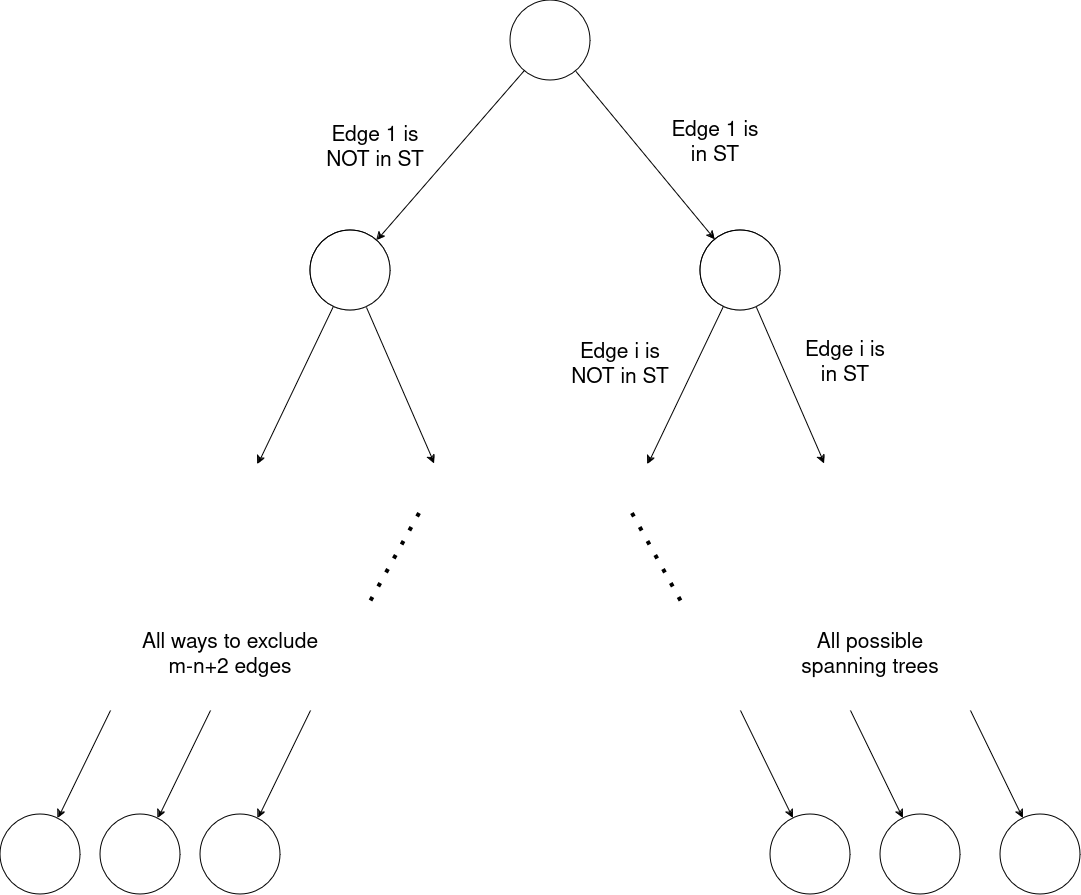
\includegraphics[width=0.8\linewidth]{Latex/Billeder/recursion_tree.png}
    \caption{Recursion tree of the brute force function. }
    \label{fig:rec_tree}
\end{figure}

In each call of the \texttt{brute\_force} function, if it is not in a base case (i.e. not a leaf in the tree) it will always make a call to itself without edge $e_i$ and if edge $e_i$ does not create a cycle so far, it will also make a call including edge $e_i$. It takes $O(\log^2(n))$ time to check for a cycle using a dynamic connectivity data structure. If the number of internal nodes in the recursion tree is $I$, this contributes $O(I\cdot\log^2(n))$ to the running time. 

In the base case, either ST consists of $n-1$ edges and there is a valid spanning tree, or there have been excluded $m-n+2$ edges and no spanning tree is possible. In the first case, the value of the spanning tree is computed and the tree is saved, taking $O(n)$ time. In the second case, the empty set is returned, taking $O(1)$ time. Worst case, this takes $O(n)$ time for each leaf node in the tree. 

In the recursion tree, a call reaches a leaf node after having either selected $n-1$ edges or excluded $m-n+2$ edges. Imagine starting at the top of the tree and going down a path to a leaf node. When including an edge $e_i$ in ST at depth $i$, go right and when excluding the edge, go left. The path stops after going right $n-1$ times or left $m-n+2$ times. Combinatorics gives that the number of unique paths is then upper bounded by
\[
    \binom{n-1+m-n+2}{n-1} = \binom{m+1}{n-1}. 
\]
This is the upper bound for the number of leaf nodes in the tree. And since each internal node in the tree at most has two children, this is also an upper bound for the number of internal nodes. 

Our analysis then gives the total running time of the brute force function as
\[
    O\left(\binom{m+1}{n-1} \cdot \left(\log^2(n) + n\right)\right) = O\left(\binom{m+1}{n-1}\cdot n\right).
\]

And since the other two steps were polynomial in running time, this is also the complexity the algorithm as a whole. 
